\newpage
\section{Training neural network models with single hidden layer}

\begin{figure}[htbp]
\centering
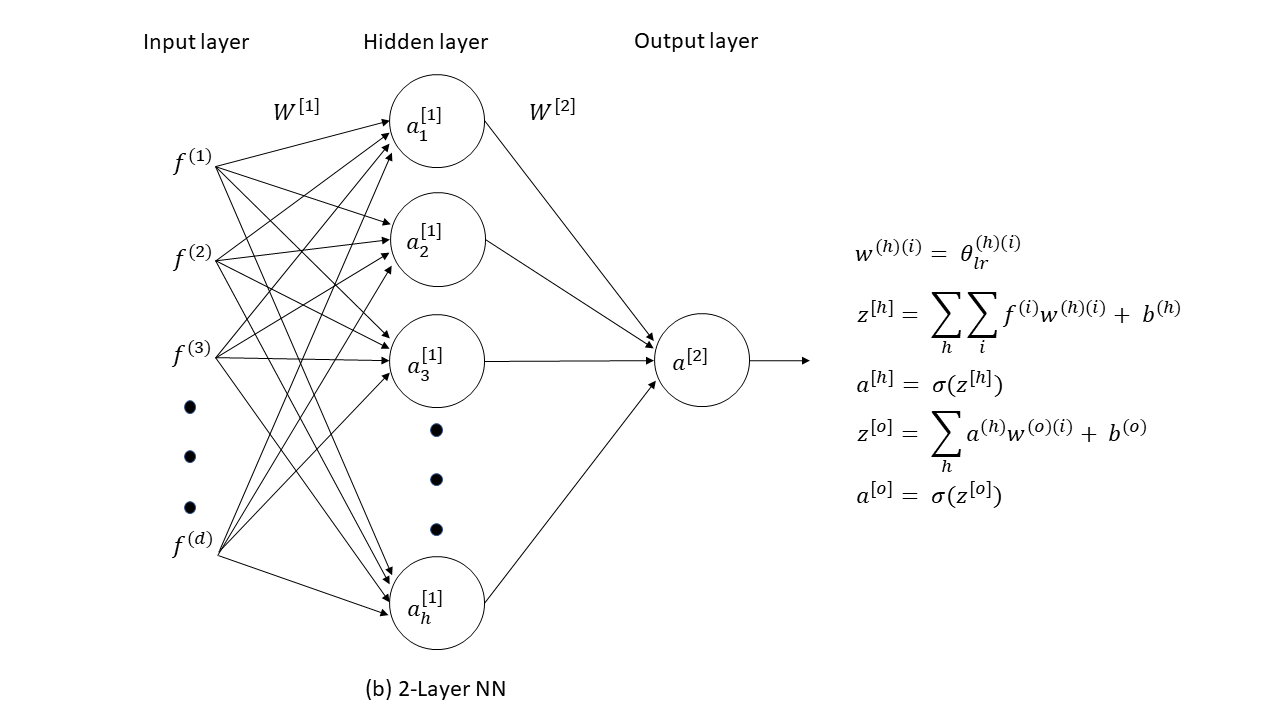
\includegraphics[width=16cm, height=10cm]{images/nn1.png}\\
\centering
\caption{Neural network model - without using word-vectors}
\label{fig:foo}
\end{figure}

\begin{figure}[htbp]
\centering
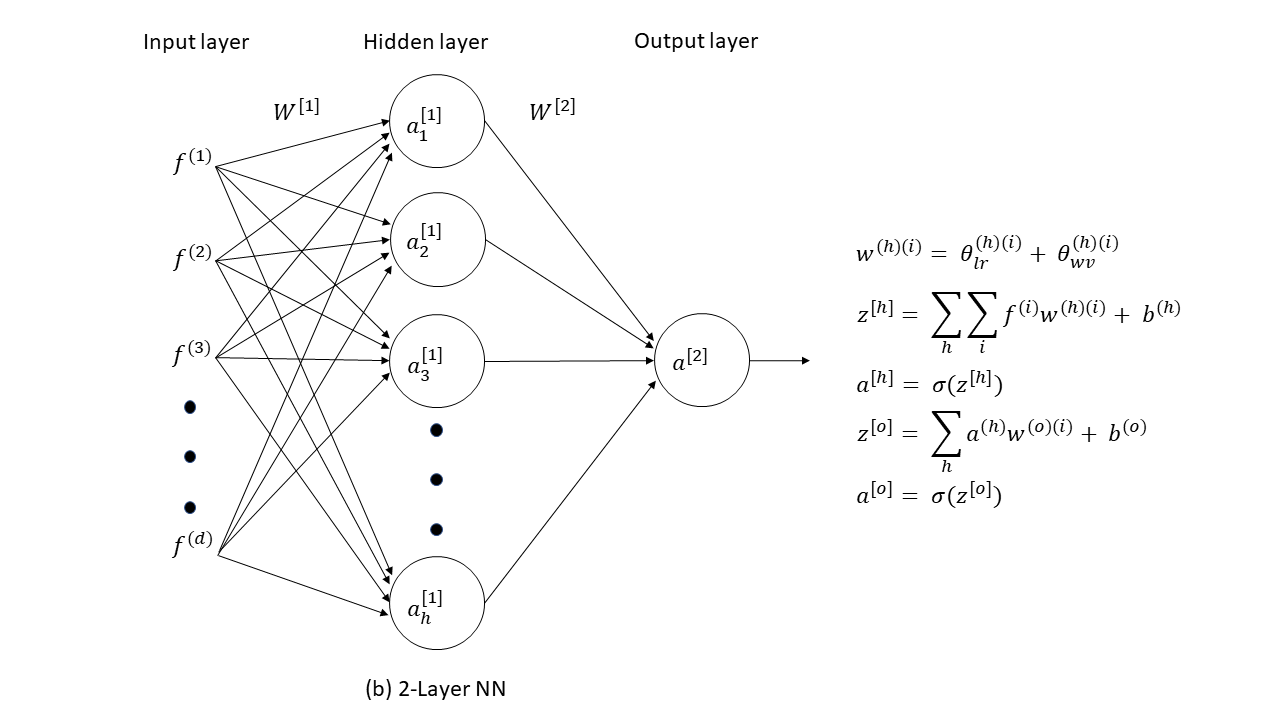
\includegraphics[width=16cm, height=10cm]{images/nn2.png}\\
\centering
\caption{Neural network model - with word-vectors}
\label{fig:foo}
\end{figure}

\newpage
\subsection{Model Performance}

Below is a table showing how a neural network model with one hidden layer performed with and without using features generated by word-vectors.

\begin{table}[htbp]
\centering
\begin{tabular}{llllll}
\multicolumn{1}{l|}{Datasets}    & \multicolumn{1}{c|}{\begin{tabular}[c]{@{}c@{}}1 layer NN\\ Set Accuracy\end{tabular}} & \multicolumn{1}{c|}{\begin{tabular}[c]{@{}c@{}}1 layer NN with wv\\ Set Accuracy\end{tabular}} &  &  &  \\ \cline{1-3}
\multicolumn{1}{l|}{IMDb}        & \multicolumn{1}{c|}{13.2}                                                              & \multicolumn{1}{c|}{19.63}                                                                     &  &  &  \\
\multicolumn{1}{l|}{20NewsGroup} & \multicolumn{1}{c|}{49.23}                                                                  & \multicolumn{1}{c|}{59.89}                                                                     &  &  &  \\
\end{tabular}
\caption{\label{tab:widgets}Set-Accuracy Results}
\end{table}


\begin{table}[htbp]
\centering
\begin{tabular}{llllll}
\multicolumn{1}{l|}{Datasets}    & \multicolumn{1}{c|}{\begin{tabular}[c]{@{}c@{}}1 layer NN\\ Instance F1\end{tabular}} & \multicolumn{1}{c|}{\begin{tabular}[c]{@{}c@{}}1 layer NN with wv\\ Instance F1\end{tabular}} &  &  &  \\ \cline{1-3}
\multicolumn{1}{l|}{IMDb}        & \multicolumn{1}{c|}{51.13}                                                            & \multicolumn{1}{c|}{60.21}                                                                    &  &  &  \\
\multicolumn{1}{l|}{20NewsGroup} & \multicolumn{1}{c|}{48.71}                                                                 & \multicolumn{1}{c|}{58.97}                                                                    &  &  &  \\
\end{tabular}
\caption{\label{tab:widgets}Instance F1 Results}
\end{table}

We can see that for both the datasets, the neural network model using features generated by word-vectors is the better performing model. In fact this model even outperforms all other previously tested models.
